\documentclass[fleqn]{article}

%\pgfplotsset{compat=1.17}

\usepackage{mathexam}
\usepackage{amsmath}
\usepackage{amsfonts}
\usepackage{graphicx}
\usepackage{systeme}
\usepackage{microtype}
\usepackage{multirow}
\usepackage{pgfplots}
\usepackage{listings}
\usepackage{tikz}
\usepackage{dsfont} %Numeros reales, naturales...
\usepackage{cancel}
\usepackage{verbatim} %comentarios de parrafos

%\graphicspath{{images/}}
\newcommand*{\QED}{\hfill\ensuremath{\square}}

%Estructura de ecuaciones
\setlength{\textwidth}{15cm} \setlength{\oddsidemargin}{5mm}
\setlength{\textheight}{23cm} \setlength{\topmargin}{-1cm}



\author{David García Curbelo}
\title{Topología}

\pagestyle{empty}


\def\R{\mathds{R}}
\def\Z{\mathds{Z}}
\def\N{\mathds{N}}
\def\S{\mathds{S}}

\def\sup{$^2$}

\def\next{\quad \Rightarrow \quad}

\begin{document}

    \setcounter{page}{1}
    \pagestyle{plain}

    \begin{center}
        {\large\bf{Topología II}} \\
        \bf{David García Curbelo}\\
        
    \end{center}

    \textbf{Ejercicio 7. } \textit{Construir una aplicación recubridora de dos hojas $\pi : C \rightarrow M$, donde C es el cilindro y M es 
            la cinta de Möbius infinita:}
            $$M = ([0,1] \times \R)/\sim, \text{ donde } (x,y) \sim (x',y') \Leftrightarrow 
            \left\{  
                \begin{aligned}
                    (x,y) &= (x',y') \\
                    &\thinspace \text{ó} \\
                    \{x,x'\} &= \{0,1\} \thinspace, \thinspace y = -y'\\
                \end{aligned}
            \right.$$
            \textit{Deducir que $\R^2$ es el recubridor universal de M.}\\

    
    Durante el ejercicio denotaremos por $\sim_{R_M}$ a la relación de equivalencia dada en el enunciado.
    Ya que el enunciado nos proporciona el conjunto $M$ en forma de conjunto cociente, comencemos considerando el conjunto $C$ del cilindro 
    también como un conjunto cociente, que lo definiremos de la siguiente manera:
    $$ C \overset{homeo}{\cong} \left([0,1] \times \R\right) / \sim_{R_C}, \quad \quad \text{donde se tiene} \quad \quad (x,y) \sim_{R_C} (x',y') \Leftrightarrow 
    \left\{ 
        \begin{aligned}
            (x,y) &= (x', y')\\
            &\text{ó}\\
            \{x,x'\} &= \{0,1\}, \thinspace \thinspace y'=y
        \end{aligned}
    \right.$$

    \begin{center}
        \noindent
        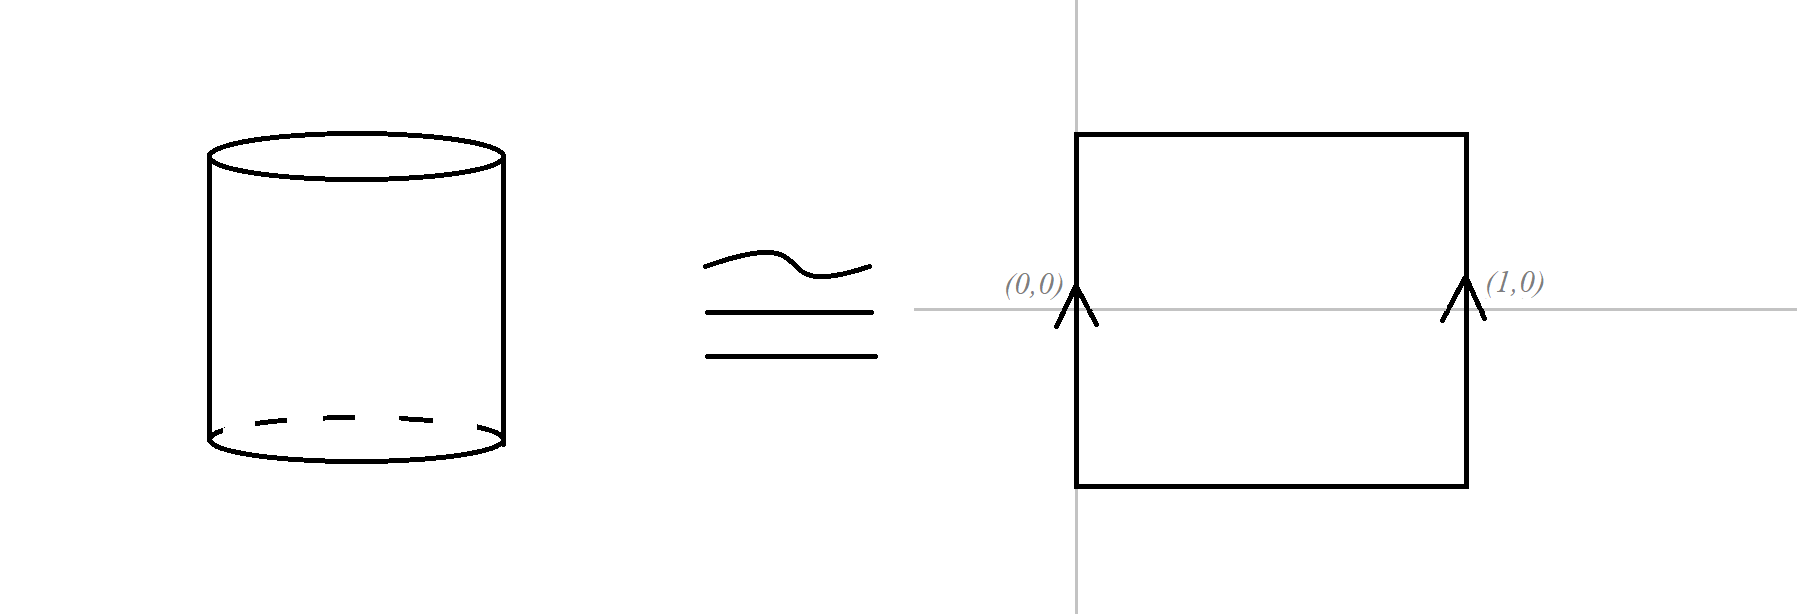
\includegraphics[width=0.6\linewidth]{cilindro.png}
    \end{center}
    
    Vemos que de la misma manera, tenemos el homeomorfismo dado en el enunciado $M \cong ([0,1] \times \R)/\sim_{R_M}$ en el que podemos ver la relación
    entre el conjunto $M$ y su conjunto cociente:
    
    \begin{center}
        \noindent
        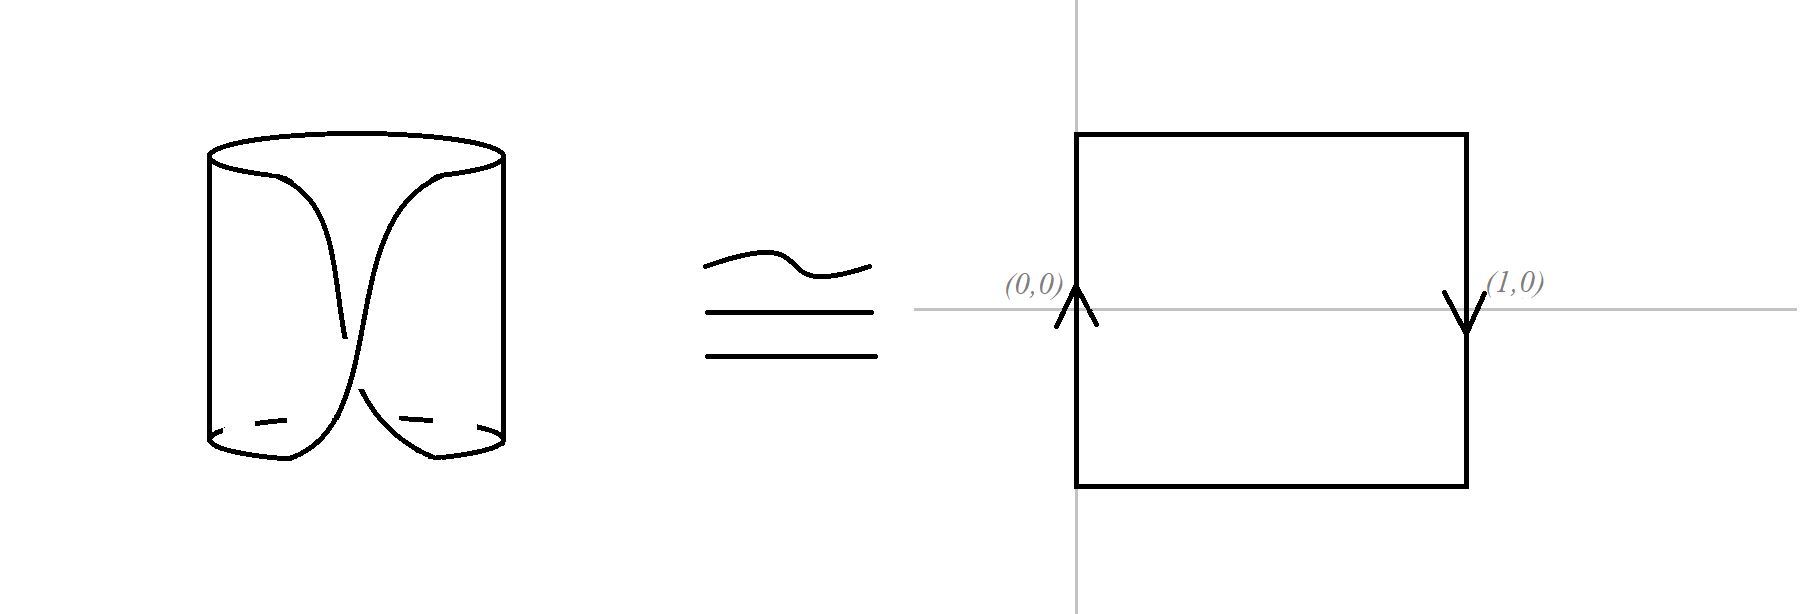
\includegraphics[width=0.6\linewidth]{moebius.png}
    \end{center}

    Por supuesto en ambas imágenes se han dibujado los bordes superiores e inferiores, pero es una simple representación para una mejor comprensión. 
    Ambas figuras son infinitas en este sentido. Ahora, teniendo los dos conjuntos cocientes, el problema se restringe a encontrar una aplicación 
    recubridora $\pi: \left([0,1] \times \R\right) / \sim_{R_C}  \rightarrow  ([0,1] \times \R)/\sim_{R_M} $. Para ello, vamos a definir previamente 
    un nuevo conjunto cociente, dado por 

\newpage

    $$ X = \left([0,2] \times \R\right) / \sim_{R_1}, \quad \quad \text{donde se tiene} \quad \quad (x,y) \sim_{R_1} (x',y') \Leftrightarrow 
    \left\{ 
        \begin{aligned}
            (x,y) &= (x', y')\\
            &\text{ó}\\
            \{x,x'\} &= \{0,2\}, \thinspace y'=y\\
            &\text{ó}\\
            \{x,x'\} &= \{0,1\}, \thinspace y'=-y\\
            &\text{ó}\\
            \{x,x'\} &= \{1,2\}, \thinspace y'=-y
        \end{aligned}
    \right.$$

    \begin{center}
        \noindent
        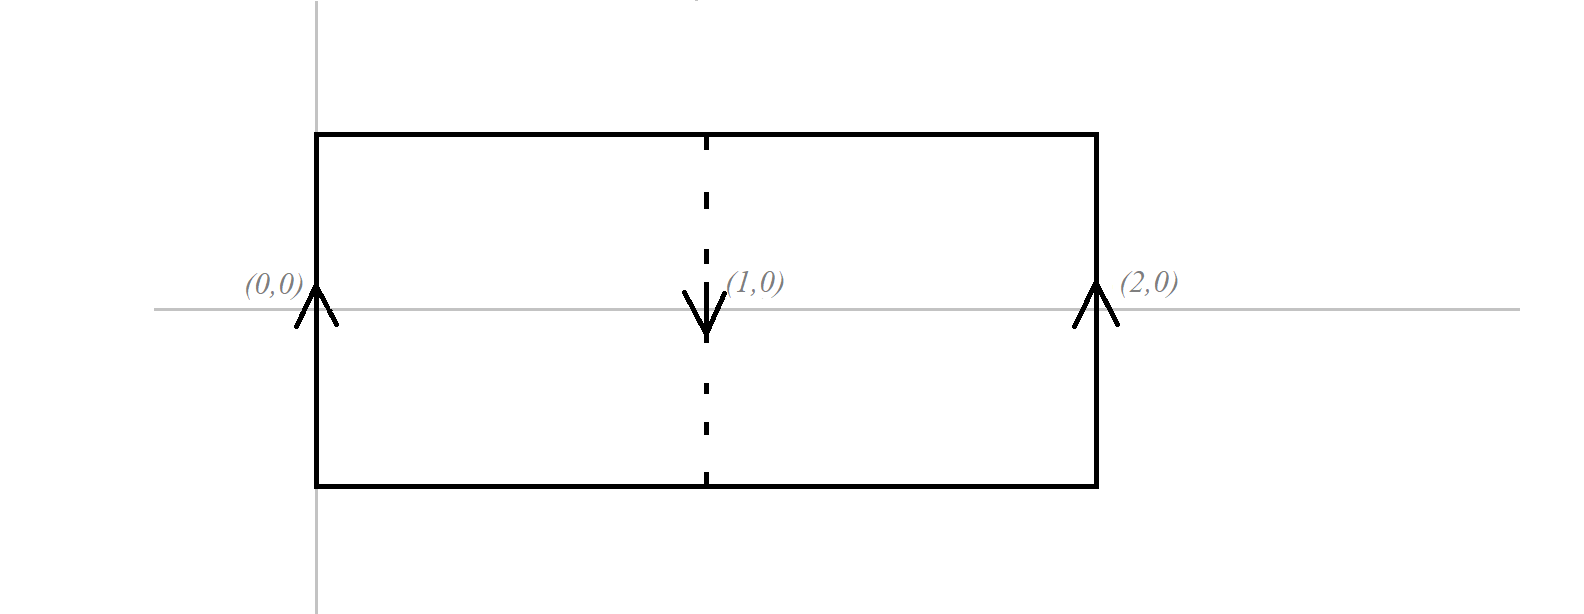
\includegraphics[width=0.6\linewidth]{doble cilindro.png}
    \end{center}
    
    Podemos considerar así la aplicación $\pi_1: C \rightarrow X$ dada por $\pi_1(x,y)=(2x,y)$ la cual es claramente continua y sobreyectiva. De la misma manera
    podemos también considerar la aplicación $\pi_2 : X \rightarrow M$ (también continua y sobreyectiva) dada por

    $$\pi_2 (x,y) = 
    \left\{
        \begin{matrix}
            \relax [(x,y)]_{R_M} \quad &\text{si }& \quad x \in (0,1)\\
            \relax [(0,-y)]_{R_M} \quad &\text{si }& \quad x = 1\\
            \relax [(x-1,y)]_{R_M} \quad &\text{si }& \quad x \in (1,2)\\
            \relax [(0,y)]_{R_M} \quad &\text{si }& \quad x \in \{0,2\}
        \end{matrix}
    \right.$$

    \begin{center}
        \noindent
        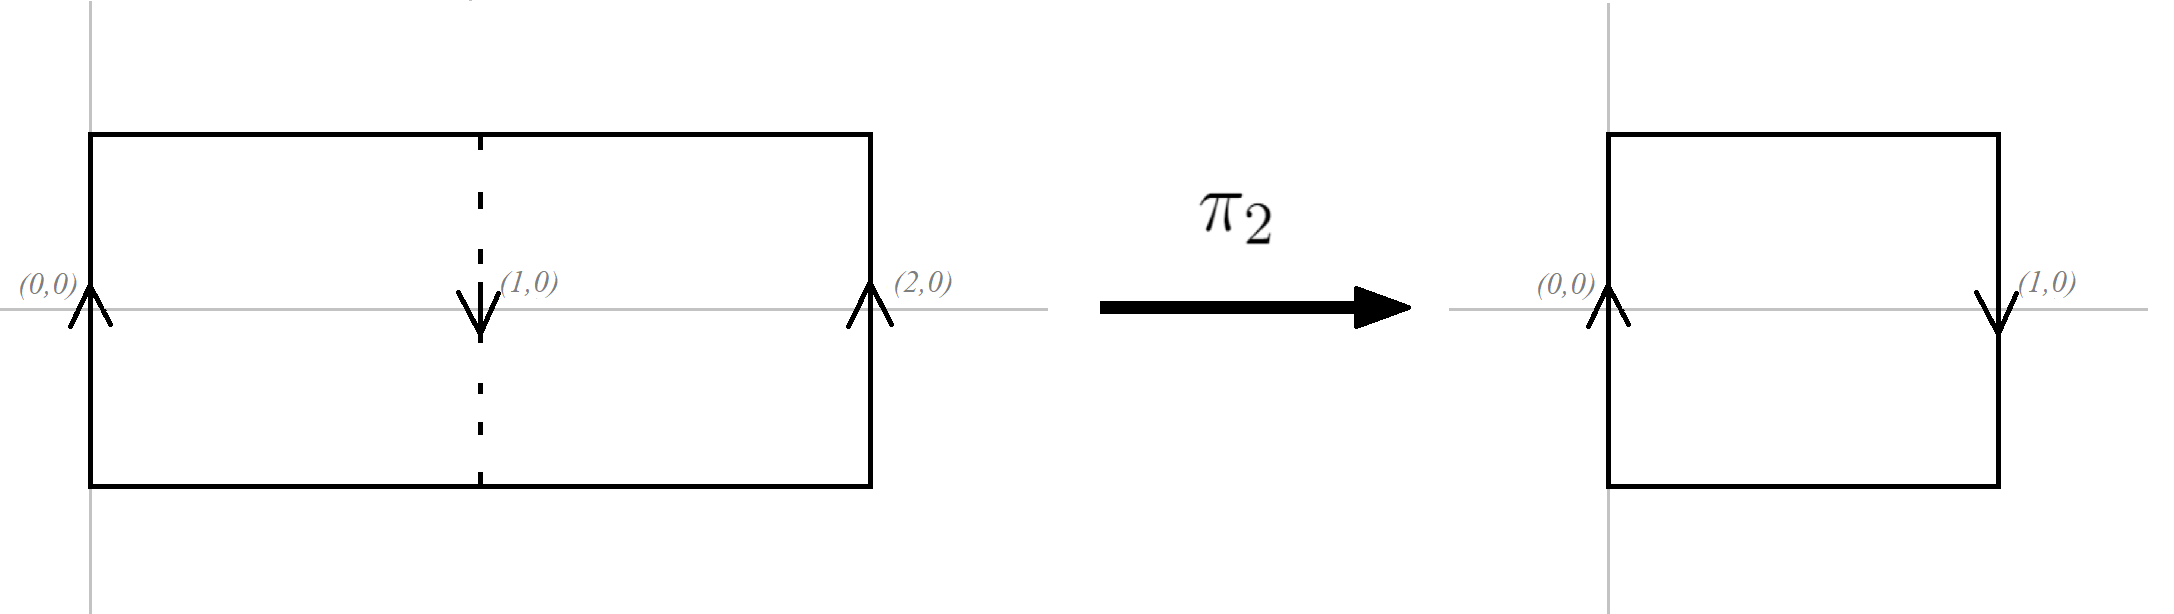
\includegraphics[width=0.6\linewidth]{pi_2.png}
    \end{center}

    Por lo tanto, la aplicación $\pi$ que andábamos buscando no es más que la composición de las dos aplicaciones que acabamos de definir, tales que
    $\pi = \pi_2 \circ \pi_1 : C \rightarrow M$. Comprobemos que verdaderamente es una aplicación recubridora. Es claro que, al ser composición de 
    aplicaciones continuas y sobreyectivas, la aplicación $\pi$ también resultará continua y sobreyectiva. Estudiemos ahora los entornos distinguidos. 
    Para ello consideremos un elemento $p = [(x,y)]_{R_M} \in M$,  distinguiremos dos casos:

\newpage

    \begin{enumerate}
        \item[\textbf{Caso 1: }] $x \in (0,1)$. En este caso tendríamos que $p = [(x,y)]_{R_M} = \{(x,y)\}$. Consideremos así un entorno $U = B((x,y), r)$ con $r>0$ lo
                            suficientemente pequeño para que no llegue al borde de nuestro conjunto. Estudiando la preimagen de nuestro elemento $p$ tenemos
                            $\pi_2 ^{-1} (p) = \{(x,y), (x+1, y)\}$, donde $ [(x,y)]_{R_1} \neq [(x+1,y)]_{R_1}$. Como sabemos que $\pi_2$ es continua, tenemos que 
                            $\pi_2 ^{-1} (U)$ es un entorno abierto tanto de $ [(x,y)]_{R_1} $ como de $ [(x+1,y)]_{R_1}$. 
                            Volviendo a realizar el mismo proceso con $\pi_1$, tenemos $\pi_1 ^{-1} \left( [(x,y)]_{R_1} \right) = [(\frac{x}{2},y)]_{R_C}$
                            y $\pi_1 ^{-1} \left( [(x+1,y)]_{R_1} \right) = [(\frac{x+1}{2},y)]_{R_C}$. Por la misma razón enunciada antes, 
                            $\pi_1^{-1}\left( \pi_2^{-1} (U)\right)$ son dos entornos abiertos (distintos) de los elementos $[(\frac{x}{2},y)]_{R_C}$ y
                            $[(\frac{x+1}{2},y)]_{R_C}$. 
                            \begin{center}
                                \noindent
                                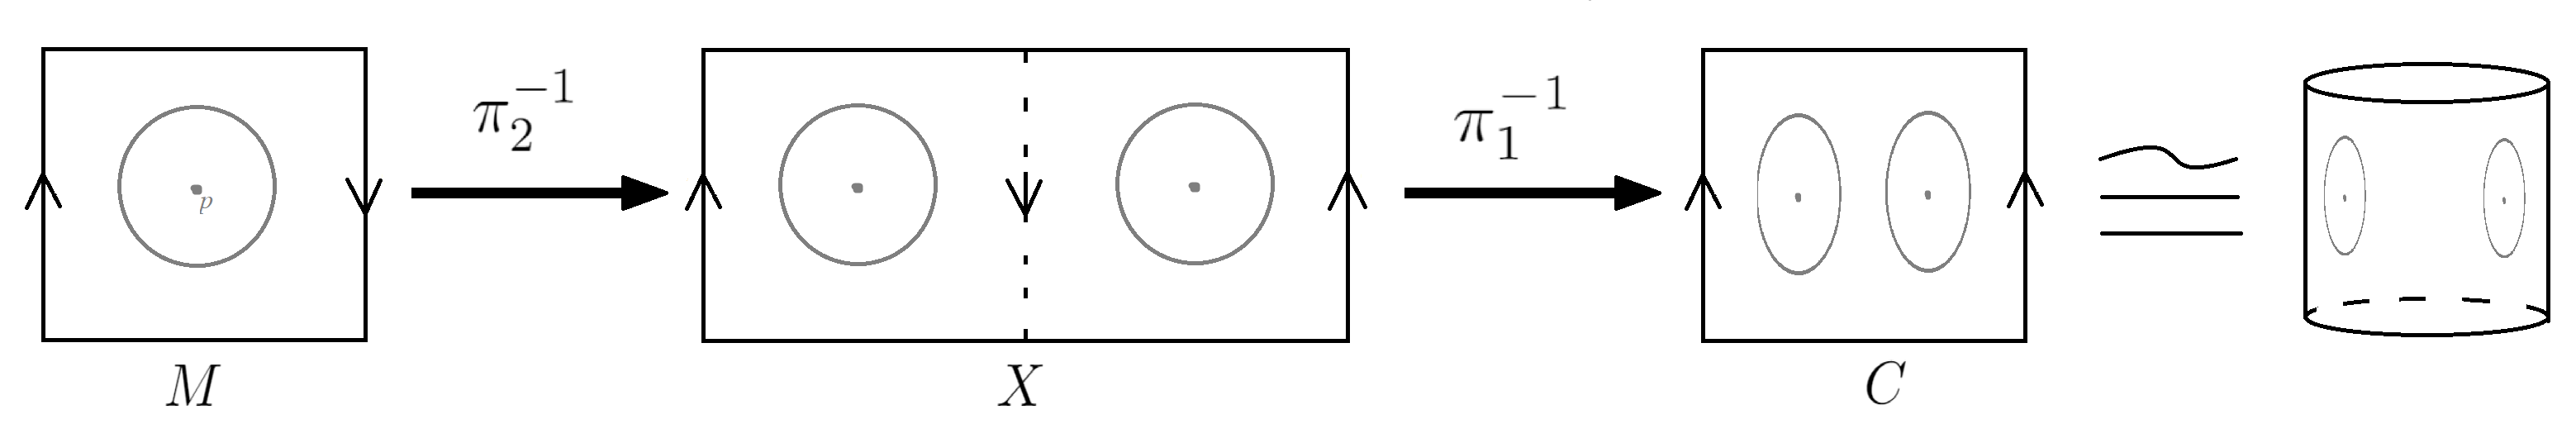
\includegraphics[width=1\linewidth]{caso1.png}
                            \end{center}
        \item[\textbf{Caso 2: }] $x \in \{0,1\}$. En este caso tendríamos que $p = [(x,y)]_{R_M} = \{(0,y),(1,-y)\}$. Consideremos ahora un entorno 
                            $U = \left( B((0,y), r) \cup B((1,-y), r)\right) \cap ([0,1] \times \R)$, con $r>0$ lo suficientemente pequeño. Realizamos ahora 
                            el mismo proceso del caso anterior. Vemos que $\pi_2 ^{-1} (p) = \{(0,y), (1,-y), (2, y)\} = [(0,y)]_{R_1}$, y como $\pi_2$ es
                            continua, se tiene que $\pi_2 ^{-1} (U)$ es un entorno abierto.
                            Tomando ahora $\pi_1$ tenemos $\pi_1 ^{-1} \left( [(0,y)]_{R_1} \right) = \{(0,y), (\frac{1}{2}, -y), (1,y)\} = \left\{[(0,y)]_{R_C}, [(\frac{1}{2},-y)]_{R_C}\right\}$.
                            Así, como $\pi_1$ es continua, tenemos que $\pi_1^{-1}\left( \pi_2^{-1} (U)\right)$ son dos entornos abiertos (distintos) de los 
                            dos elementos que hemos obtenido.
                            \begin{center}
                                \noindent
                                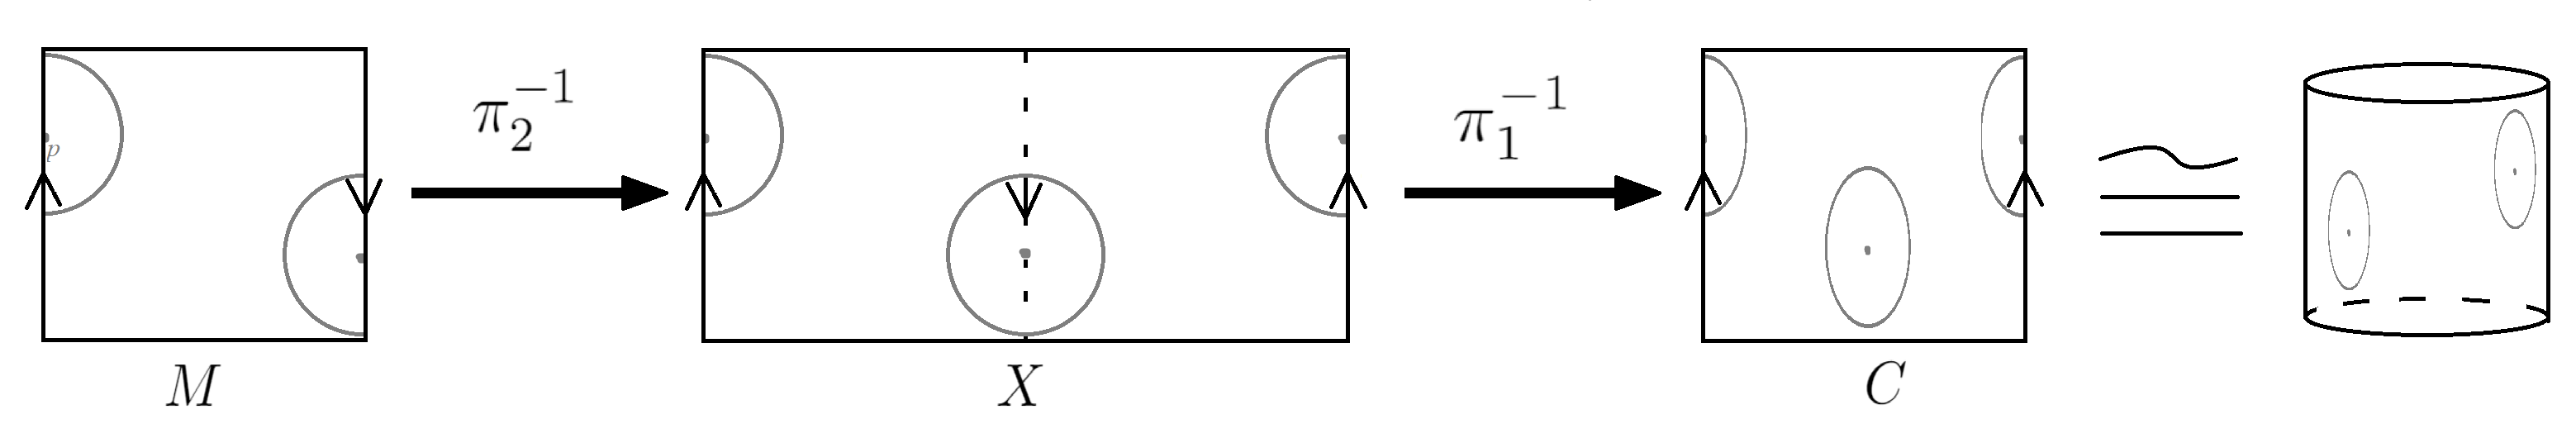
\includegraphics[width=1\linewidth]{caso2.png}
                            \end{center}
    \end{enumerate}

    Con esto hemos demostrado que nuestra aplicación $\pi$ es una aplicación recubridora, y efectivamente de dos hojas, ya que se cumple que 
    $Card(\pi^{-1}\left( \left[ \left( x,y \right) \right]_{R_M} \right)) = 2$, $\forall (x,y) \in C$, luego tenemos lo que buscábamos.


    Veamos ahora que $\R^2$ es efectivamente el recubridor universal de $M$. Ya que $\R^2$ es simplemente conexo, si es recubridor forzosamente será también 
    recubridor universal. Encontremos primero un espacio recubridor $(\phi, \R^2)$ de $C$. Para ello basta con ver que, como la aplicación exponencial $\rho$ 
    es una aplicación recubridora de $\R$ sobre $\S^1$, es claro que $(\rho \times \text{Id}_{\R}, \R^2)$ es un espacio recubridor de $\S^1 \times \R = C$. 
    Teniendo esto así, podemos considerar $(\pi \circ (\rho \times \text{Id}_{\R}), \R^2)$ el espacio recubridor de $M$ ,y además, por ser simplemente conexo y 
    $\Pi_1 (\R^2) \cong \{1\}$, tenemos que efectivamente $\R^2$ es el recubridor universal de $M$.

\end{document}